\chapter{Modal Reduction}

\renewcommand\scaleBlade{0.64}

The following sections aim to explain the dimensionality reduction of the problem comparing the \textbf{Kulfan} based representation of the domain 
to a more \textbf{physical} representation using a \textbf{modal decomposition} of data. 

\section{Problem Framing}

The principal component analysis is one of the main methods for the dimensionality reduction of a problem~\cite{geron2022hands}. 
Unlike the machine learning part, the study is conducted only over the $\mathcal{Y}$ dataset. 

\section{Principal Component Analysis}

The method starts with a global analysis of the correlation between the different blade parameters:

\begin{itemize}
    \item $\gamma$, $\chi_1$ and $\chi_2$ for the camberline
    \item $A_{suct}$ for the suction side parametrization
    \item $A_{press}$ for the pressure side parametrization
    \item $pitch$
\end{itemize}

From this correlation analysis, the method extracts the main correlation directions. 
These directions will then define a vector which can be seen as one of the eigenvectors which defines the $\mathcal{Y}$ dataset.
After having computed the first direction, it is possible to compute the other \textit{modal directions}.

Listing~\ref{listing:PCA} shows the code used for the the principal component analysis of the $\mathcal{Y}$ dataset.

\lstinputlisting[style=customPy, caption=PCA decomposition, label=listing:PCA]{./code/PCA.txt}

Once computed all the \textit{modal directions}, it is possible to understand their importance for the 
definition of the whole dataset. For each \textit{modal direction} a variance index can be extracted.
This index represents the importance of the mode in the whole database. 
The higher the variance the higher the dataset coverage of its respective \textit{mode}.

A good dataset coverage is presented for a variance coverage above of $95\%$. 

Figure~\ref{fig:PCA} shows the variance distribution related to the dataset modes. 
With \textit{just} three modes it is possible to cover more than $95\%$ of the entire database.

\begin{figure}[H]
    \centering
    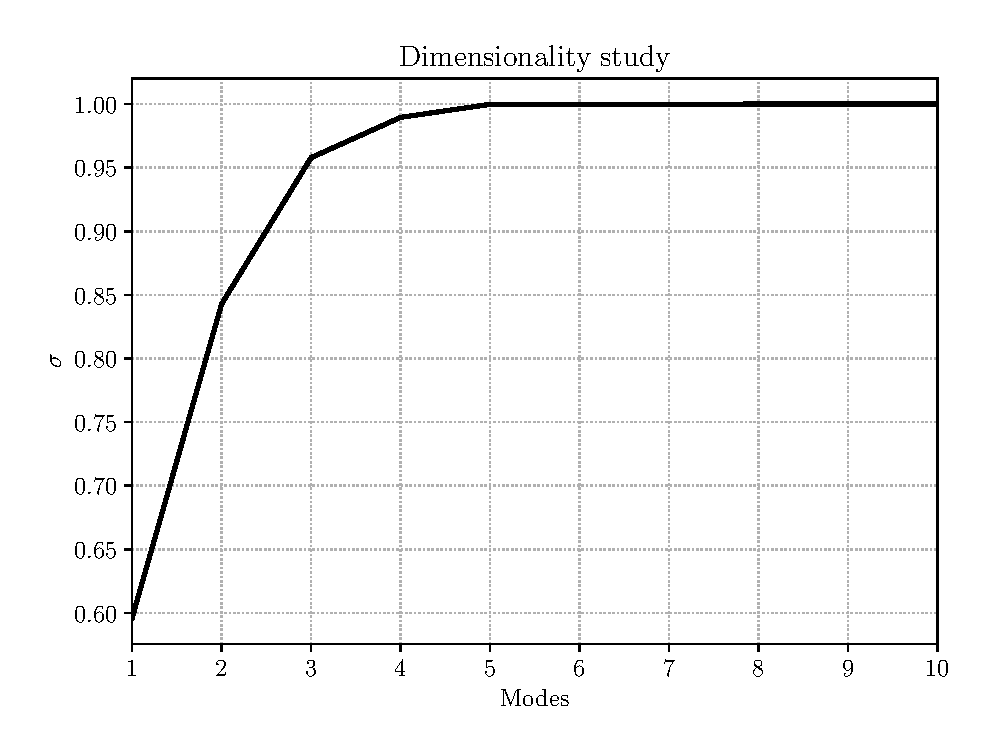
\includegraphics[scale=0.7]{./images/PCAmodes.eps}
    \caption{Principal Components of $\mathcal{Y}$ dataset.}
    \label{fig:PCA}
\end{figure}

\subsection{Modal Analysis}

% Having studied the main modes of $\mathcal{Y}$, it is possible to relate the load 
% variation due to these modes. This step allows to filter, again, the domain of study 
% passing through \textit{just} one dataset, $\mathcal{Y}$. This filtering action 
% does not have a direct corrleation to the $\mathcal{X}$ dataset but it can be seen better
% as the direct output of the main geometrical features of the $\mathcal{Y}$ dataset.

After analyzing the primary modes within $\mathcal{Y}$, it becomes feasible to establish a connection between the load variations attributed to these modes. This procedure facilitates a further refinement of the study domain by solely considering a single dataset, namely $\mathcal{Y}$. This filtering process is not directly linked to the $\mathcal{X}$ dataset; instead, it can be better understood as a direct manifestation of the key geometric characteristics inherent in the $\mathcal{Y}$ dataset.

Figure~\ref{fig:PCAmode1} shows the first mode. This mode is represented 
letting varying its amplitude over a reference blade. Figure~\ref{fig:PCAmode1}
represents also the load distribution varying the mode amplitude. From the plot 
it is possible understand that the first mode comprehends a lot of variation of the camberline.
This variation will result in a change of the suction side load, especially on the peak 
Mach number and on the leading edge loading.

\begin{figure}[H]
    \centering
    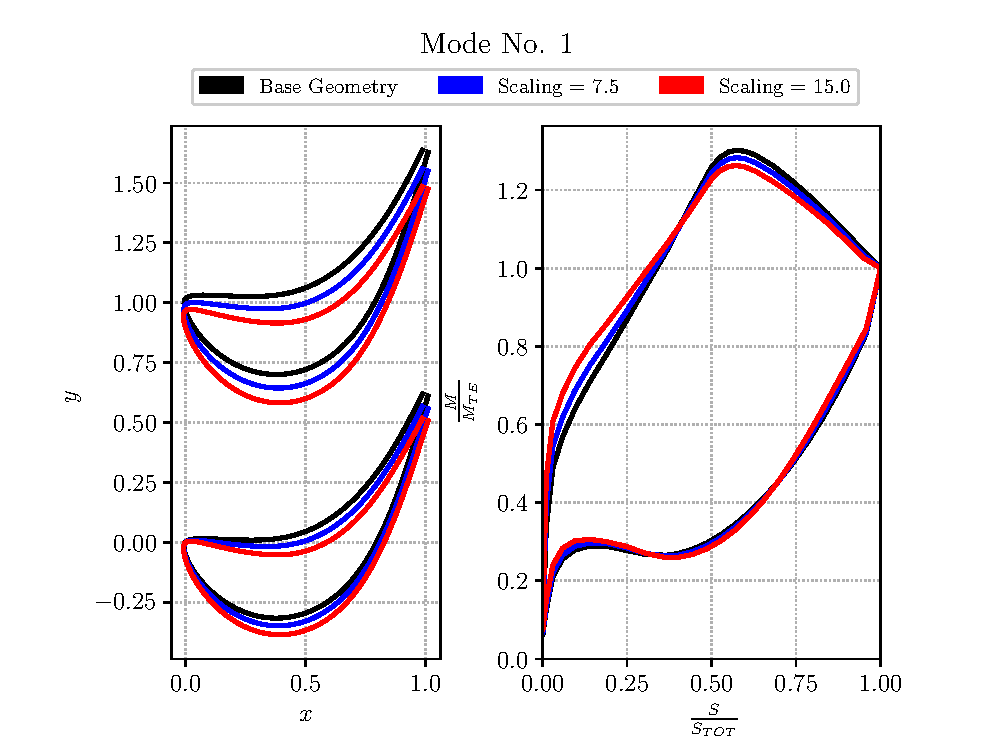
\includegraphics[scale=\scaleBlade]{./images/mode01.eps}
    \caption{Mode No. 1 with the respective modal loading distribution.}
    \label{fig:PCAmode1}
\end{figure}

\begin{figure}[H]
    \centering
    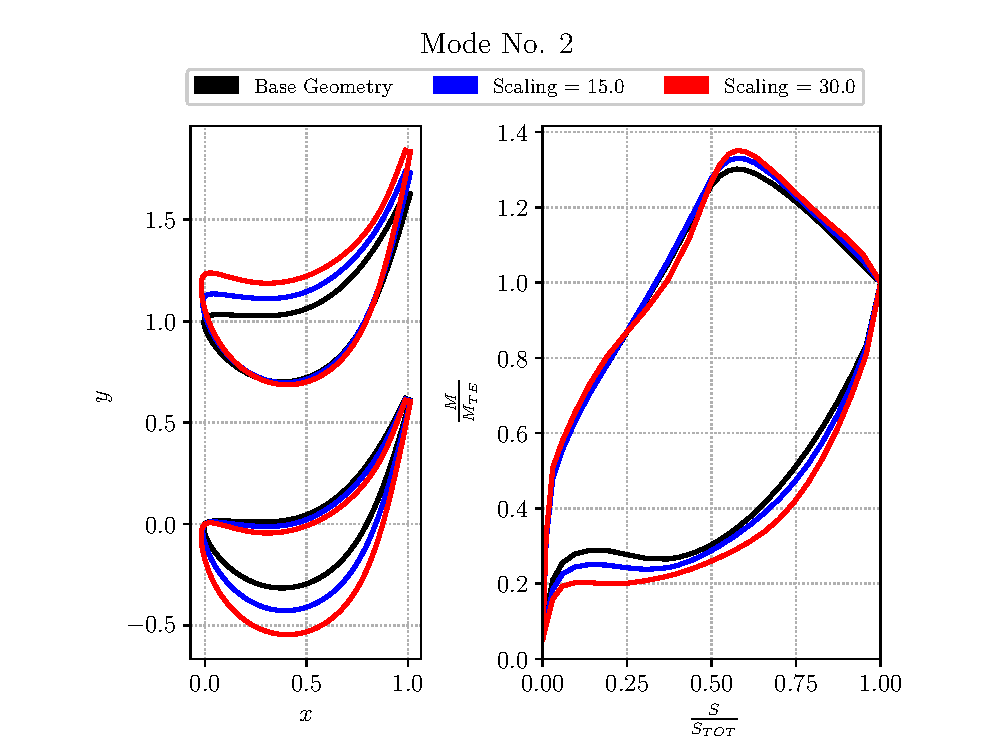
\includegraphics[scale=\scaleBlade]{./images/mode02.eps}
    \caption{Mode No. 2 with the respective modal loading distribution.}
    \label{fig:PCAmode2}
\end{figure}

The second mode, represented in Figure~\ref{fig:PCAmode2}, involves heavily the blade thickness variation.
The blade thickness variations do not change the loading at the leading edge on the suction side 
but it has an evident effect on the loading distribution at the leading edge on the pressure side. 
Even though the suction side leading edge is not affected by this mode, the peak Mach number 
on the suction side of the blade shows dependence on this mode; it can be seen as a mode 
which changes locally the load distribution over the suction side.

The first and second mode do not affect the position of the peak Mach number over the suction side.
The third mode, represented in Figure~\ref{fig:PCAmode3}, features the change in the position of the peak Mach number on the suction side. 
At the same time, appreciable changes are made on the pressure side Mach distribution.

\begin{figure}[H]
    \centering
    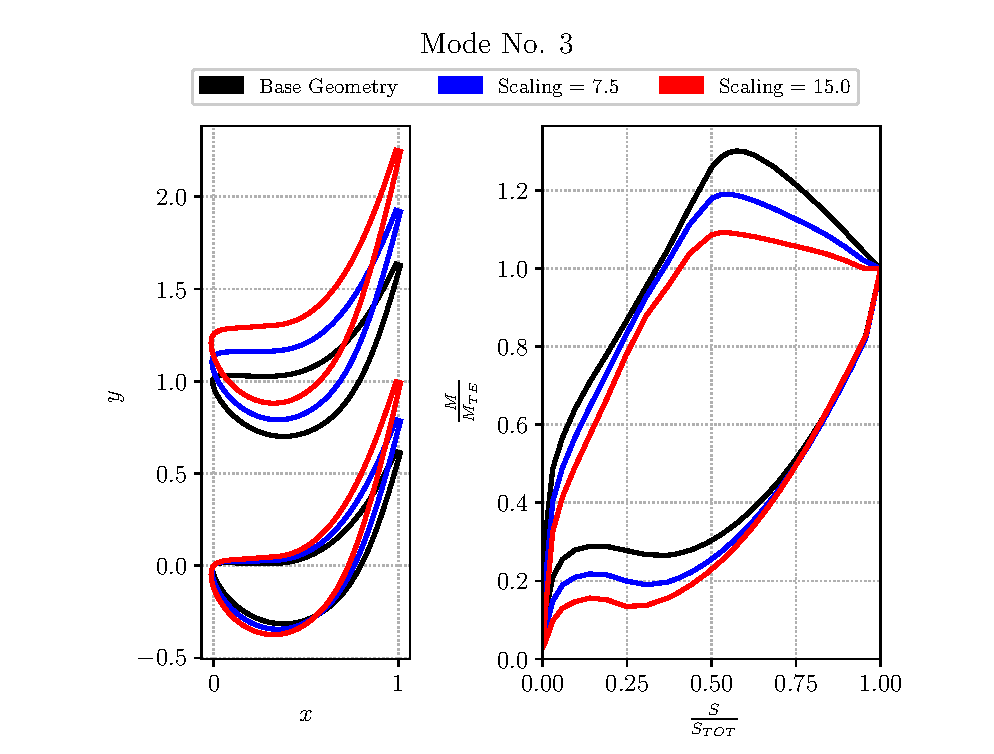
\includegraphics[scale=\scaleBlade]{./images/mode03.eps}
    \caption{Mode No. 3 with the respective modal loading distribution.}
    \label{fig:PCAmode3}
\end{figure} 

\begin{figure}[H]
    \centering
    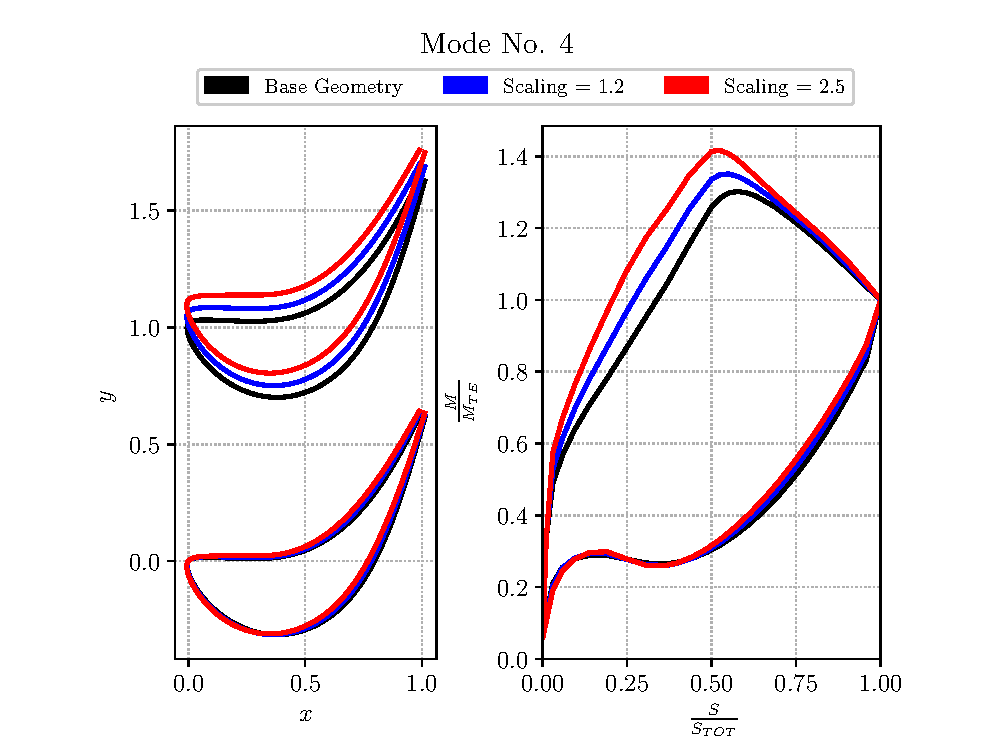
\includegraphics[scale=\scaleBlade]{./images/mode04.eps}
    \caption{Mode No. 4 with the respective modal loading distribution.}
    \label{fig:PCAmode4}
\end{figure}

Figure~\ref{fig:PCAmode4} represents the fourth dataset mode. Even though this mode can be seen as important, 
the dataset it spans is relatively small. This because the variance, $\sigma$, attributed to the fourth mode is smaller than the variance of its previous modal forms.
This mode features best the changes over the suction side of the blade. It is clear that the leading edge loading and the peak load on the suction side of the blade 
are heavily dependent on this mode. Even though this behavior, the influence of this mode on the dataset is of lower importance compared to the first mode.

\begin{figure}[H]
    \centering
    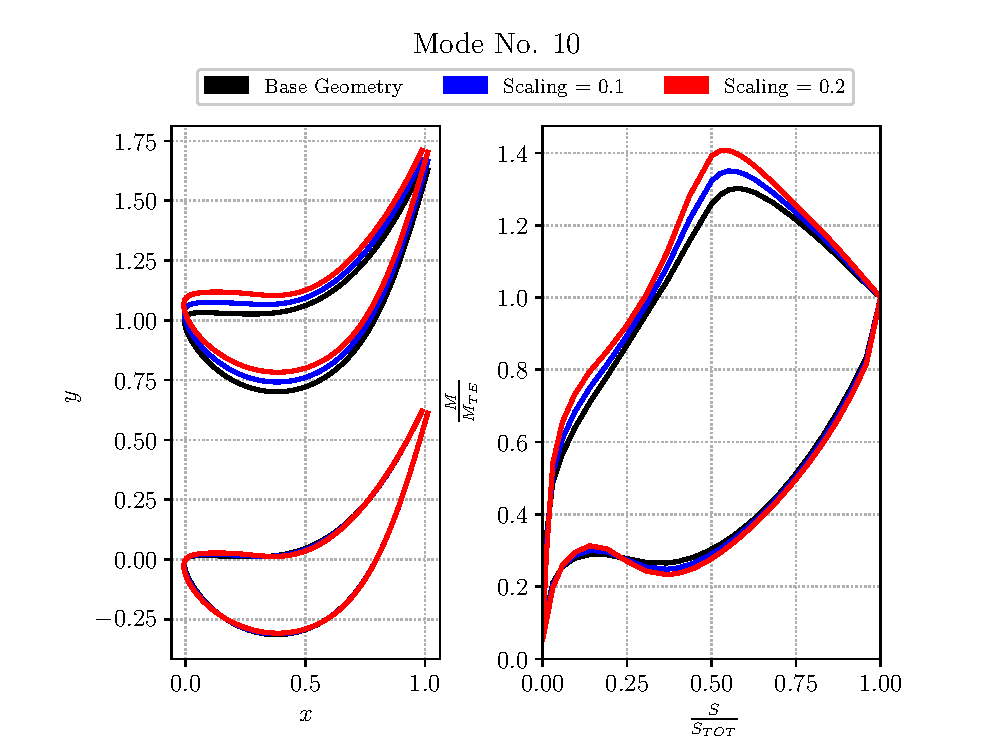
\includegraphics[scale=\scaleBlade]{./images/mode10.eps}
    \caption{Mode No. 10 with the respective modal loading distribution.}
    \label{fig:PCAmode10}
\end{figure}

The present work has shown the principal dataset modes - from the first mode to the third - but it
does not show the whole modal spectrum of the $\mathcal{Y}$ dataset. The following modes 
are more related to important modal forms from which important results can be taken. 

One of the most particular modal shapes are the 10th mode, the 30th mode and 42nd mode, the last mode.
These modes underline important physical properties:

\begin{itemize}
    \item the fact that the modal spectrum does not follow the same engineering strategy for the design of a section 
    but it relies \textbf{only} on the dataset: mode 10th.
    \item there are modes which act on a very specific part of the loading distribution: mode 30th.
    \item there are modes which can be seen as noise and have low importance in the section design process: mode 42nd.
\end{itemize}

Figure~\ref{fig:PCAmode10} shows the 10th mode. This mode affects mainly the pitch degree of freedom.
This mode changes the load distribution over the blade because a variation of the channel size. 
At the same time, the exit flow angle is heavily dependent on the solidity ($solidity = \frac{pitch}{chord}$) which is related to the pitch.

\begin{figure}[H]
    \centering
    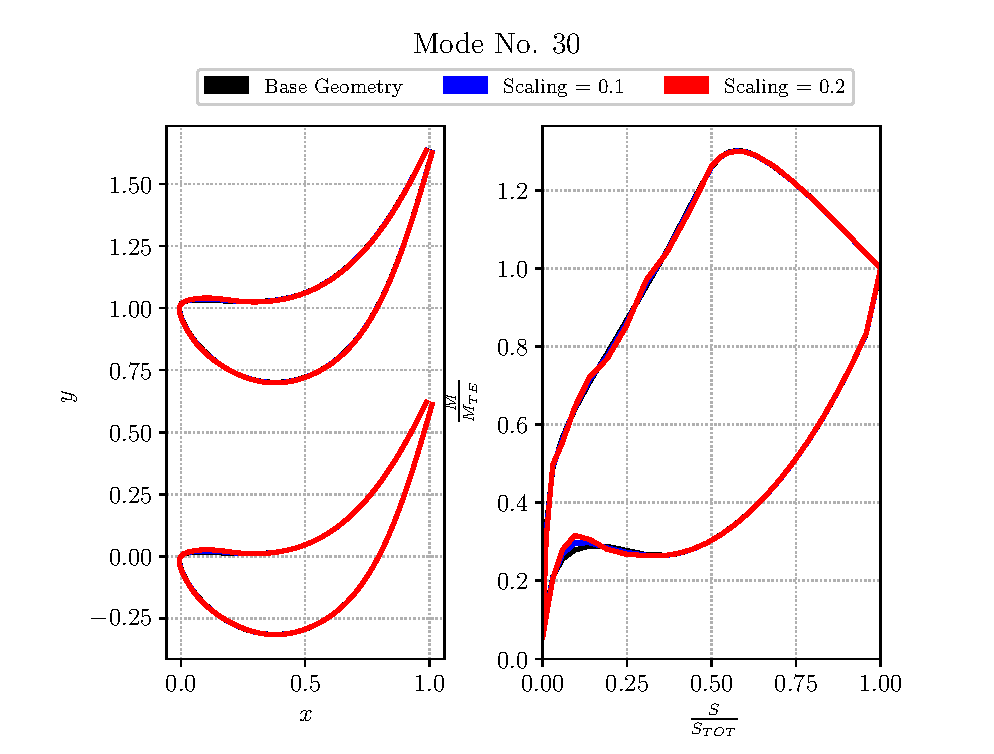
\includegraphics[scale=\scaleBlade]{./images/mode30.eps}
    \caption{Mode No. 30 with the respective modal loading distribution.}
    \label{fig:PCAmode30}
\end{figure}

Even though the 10th mode can be seen as an important mode because of the turbomachinery theory, 
it is of secondary importance inside the modal behavior of the system. This because the previous modes
\textbf{span much more space} than the 10th.

Using Figure~\ref{fig:PCAmode30}, it is possible to understand the influence, both 
over geometry and loading, of a low-variance mode. In this figure, the main geometrical 
variation is made over the pressure side at the leading edge of the blade. This change 
affects mostly the local Mach fraction distribution at the leading edge on the pressure side.
With this mode, it is possible to highlight the fact that avoiding modes with low variance 
does not generate huge errors in the geometry representation.

Figure~\ref{fig:PCAmode42} shows the last modal shape. This shape can be seen as 
a wobbling noise around the blade and it has the lowest importance in the 
representation of the blade domain. As the 30th modal shape, the 42nd mode 
can be dropped off for a modal representation of a blade without loosing accuracy
both in geometry and loading.

\begin{figure}[H]
    \centering
    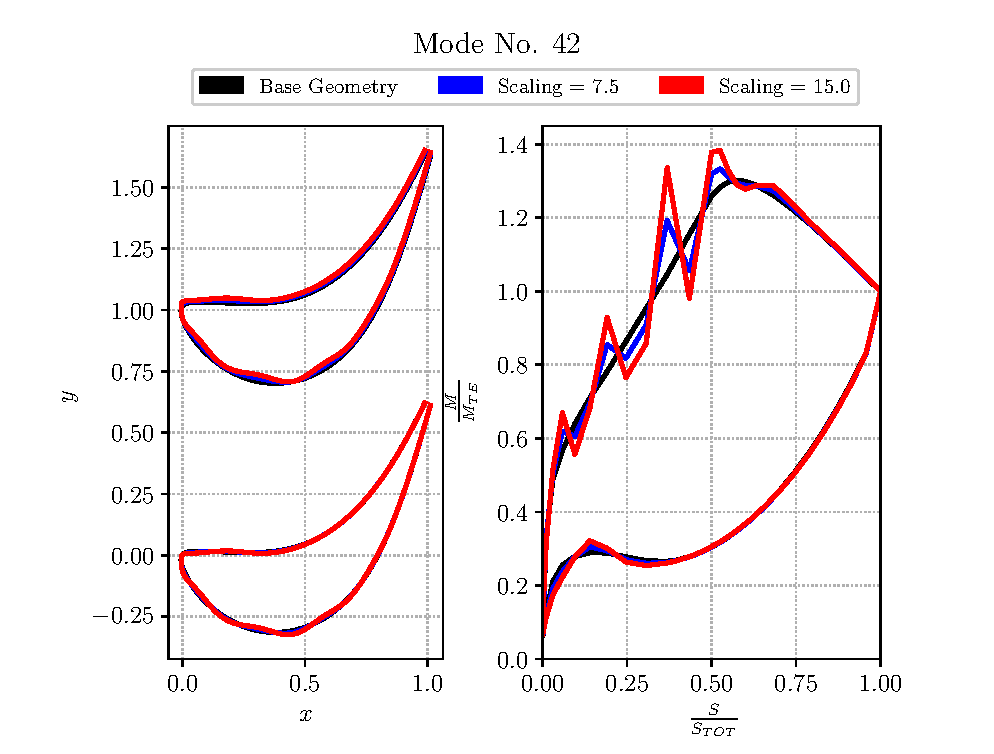
\includegraphics[scale=\scaleBlade]{./images/mode42.eps}
    \caption{Mode No. 42 with the respective modal loading distribution.}
    \label{fig:PCAmode42}
\end{figure}
